\documentclass[11pt,a4paper]{article}
\usepackage[margin=1in]{geometry}
\usepackage{amsmath,amssymb}
\usepackage{graphicx}
\usepackage{enumitem}
\usepackage{tcolorbox}
\usepackage{array}
\usepackage{multirow}
\usepackage{tikz}
\usepackage{xcolor}
\usetikzlibrary{positioning,arrows.meta,shapes}

% Custom commands
\newcommand{\highlight}[1]{\textbf{#1}}
\newcommand{\answer}[1]{\textcolor{blue}{\textit{#1}}}
\newcommand{\teaching}[1]{\textcolor{red}{\textbf{Teaching Note: }#1}}

% Box for exercises
\newtcolorbox{exercise}[1][]{
    colback=blue!5!white,
    colframe=blue!75!black,
    title=#1,
    fonttitle=\bfseries
}

\newtcolorbox{discovery}[1][]{
    colback=yellow!5!white,
    colframe=orange!75!black,
    title=Discovery Moment,
    fonttitle=\bfseries
}

\newtcolorbox{think}[1][]{
    colback=green!5!white,
    colframe=green!75!black,
    title=Think About It,
    fonttitle=\bfseries
}

\newtcolorbox{teachingnote}[1][]{
    colback=red!5!white,
    colframe=red!75!black,
    title=Teaching Note,
    fonttitle=\bfseries
}

\title{\textbf{Week 2: Teaching Computers to Understand Word Relationships}\\
\large Discovering How Machines Learn Language\\
\large Pre-Lab Exercise (No Programming Required)\\
\textcolor{red}{\textbf{INSTRUCTOR VERSION WITH ANSWER KEY}}}
\author{NLP Course 2025}
\date{}

\begin{document}
\maketitle

\noindent\textbf{Time:} 30-40 minutes\\
\textbf{Objective:} Discover three fundamental ways computers can learn word meanings from text.

\begin{teachingnote}
This handout uses discovery-based learning. Students don't know the terms CBOW, Skip-gram, or Negative Sampling yet. They will discover these concepts naturally through exercises, then learn the technical terms. Encourage exploration and ``aha!'' moments.
\end{teachingnote}

\section*{Part 1: How Words Keep Company (8 minutes)}

\begin{exercise}[Word Prediction Game]
\textbf{Task 1: Fill in the blanks with the most likely word:}
\begin{enumerate}[label=\alph*)]
    \item The cat sat on the \answer{mat/floor/couch/rug}
    \item I drink \answer{coffee/tea/water} every morning
    \item The \answer{dog} barked loudly at the mailman
    \item She wore a beautiful \answer{dress/gown/outfit} to the wedding
\end{enumerate}

\teaching{Let students share different valid answers. This shows that context allows multiple possibilities, not just one "correct" answer.}

\textbf{Task 2: Reflection}
\begin{enumerate}
    \item How did you know what words to fill in? What clues did you use?
    
    \answer{The surrounding words (context) give clues about what makes sense. Words that commonly appear together helped me predict the missing word.}
    
    \item List the words that helped you guess the answer for (a):
    
    Helper words: \answer{cat, sat, on, the (all the surrounding words)}
    
    \item \textbf{Important Discovery:} You used the surrounding words to predict the missing word. 
    
    In your own words, explain why surrounding words help:
    
    \answer{Words that appear together often have related meanings or describe common situations. The context tells us what type of word fits grammatically and semantically.}
\end{enumerate}
\end{exercise}

\begin{think}
If humans can guess words from their surroundings, can we teach computers to do the same?
\end{think}

\teaching{This is the key insight of distributional semantics - meaning comes from context!}

\section*{Part 2: Two Ways to Learn Words (10 minutes)}

\begin{exercise}[Method A: Many Words Predict One]
Imagine you're teaching a computer to fill in blanks like you just did.

\textbf{Scenario:} ``The quick brown \underline{\hspace{2cm}} jumps over''

\textbf{Task 1: Design the Learning}
\begin{enumerate}
    \item What information would you give the computer as INPUT?
    
    INPUT: \answer{The surrounding words: quick, brown, jumps, over}
    
    \item What should the computer learn to OUTPUT?
    
    OUTPUT: \answer{The missing/center word (fox, dog, cat, etc.)}
    
    \item Draw how this works (use arrows):
    \begin{center}
    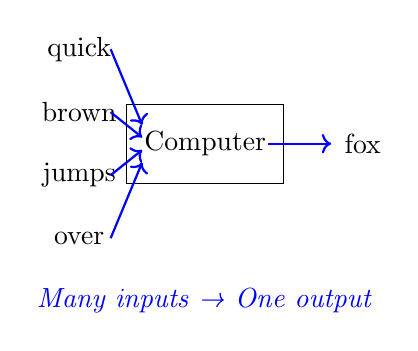
\begin{tikzpicture}[scale=0.8]
        \node at (-2, 1.5) {quick};
        \node at (-2, 0.5) {brown};
        \node at (-2, -0.5) {jumps};
        \node at (-2, -1.5) {over};
        
        \node[draw, rectangle, minimum width=2cm, minimum height=1cm] at (0, 0) {Computer};
        
        \node at (2.5, 0) {fox};
        
        % Answer arrows
        \draw[->, blue, thick] (-1.5, 1.5) -- (-1, 0.3);
        \draw[->, blue, thick] (-1.5, 0.5) -- (-1, 0.1);
        \draw[->, blue, thick] (-1.5, -0.5) -- (-1, -0.1);
        \draw[->, blue, thick] (-1.5, -1.5) -- (-1, -0.3);
        \draw[->, blue, thick] (1, 0) -- (2, 0);
        
        \node[blue] at (0, -2.5) {\answer{Many inputs → One output}};
    \end{tikzpicture}
    \end{center}
\end{enumerate}

\textbf{Task 2: Practice Examples}

Using Method A (surrounding words → missing word), predict:
\begin{enumerate}
    \item [dog, walked, the, park] → \answer{in/through/around}
    \item [ate, pizza, for, lunch] → \answer{I/we/they}
\end{enumerate}
\end{exercise}

\begin{discovery}
Congratulations! You've just invented an approach that computer scientists call ``CBOW'' (Continuous Bag of Words). It uses context words to predict a center word - just like you did!
\end{discovery}

\teaching{Emphasize that they discovered this naturally - CBOW is just a name for what they figured out!}

\begin{exercise}[Method B: One Word Predicts Many]
Now let's flip it around!

\textbf{Scenario:} Given the word ``coffee'', predict what words often appear near it.

\textbf{Task 1: Word Association}
\begin{enumerate}
    \item Given ``coffee'', list 4 words that often appear nearby:
    \begin{itemize}
        \item \answer{drink/morning/cup/hot}
        \item \answer{black/strong/fresh/brew}
        \item \answer{shop/maker/beans/mug}
        \item \answer{caffeine/espresso/latte}
    \end{itemize}
    
    \item This is the OPPOSITE of Method A. Complete:
    \begin{itemize}
        \item Method A: Many words → \answer{One word}
        \item Method B: One word → \answer{Many words}
    \end{itemize}
    
    \item Which method creates MORE training examples from one sentence? Why?
    
    \answer{Method B (Skip-gram) creates more examples. For each center word, it creates multiple training pairs (one for each context word), while CBOW creates just one example per center word position.}
\end{enumerate}
\end{exercise}

\begin{discovery}
You've discovered ``Skip-gram''! It takes one word and predicts the surrounding context - the reverse of CBOW.
\end{discovery}

\teaching{Skip-gram typically works better for rare words because it generates more training data per word occurrence.}

\section*{Part 3: Making It Faster - A Clever Trick (10 minutes)}

\begin{exercise}[The Speed Problem]
\textbf{The Challenge:} English has about 50,000 common words. Every time the computer learns, should it:
\begin{itemize}
    \item Option A: Check all 50,000 words to find the right one?
    \item Option B: Check just 5-10 words?
\end{itemize}

Obviously, Option B is faster! But how can we do this?

\teaching{Let students struggle with this briefly - the solution isn't obvious!}

\textbf{Task 1: Real or Fake?}

Instead of finding THE right word out of 50,000, let's play a simpler game:

Given word pairs, decide if they're REAL (actually appear together) or FAKE (random pairing):

\begin{center}
\begin{tabular}{|l|l|c|}
\hline
\textbf{Word 1} & \textbf{Word 2} & \textbf{Real or Fake?} \\
\hline
coffee & drink & \answer{Real} \\
\hline
coffee & elephant & \answer{Fake} \\
\hline
dog & barked & \answer{Real} \\
\hline
dog & galaxy & \answer{Fake} \\
\hline
queen & king & \answer{Real} \\
\hline
queen & bicycle & \answer{Fake} \\
\hline
\end{tabular}
\end{center}

\textbf{Task 2: Understanding the Trick}
\begin{enumerate}
    \item Instead of asking ``Which of 50,000 words is correct?'', we now ask:
    
    New question: \answer{``Is this word pair real or fake?'' (binary classification)}
    
    \item For each real pair, how many fake pairs should we create for good learning?
    
    \answer{5-10} fake pairs \teaching{Typically 5-20, with 5 being common}
    
    \item If we use 5 fake pairs + 1 real pair, we only update 6 words instead of 50,000.
    
    What's the speedup? \answer{50,000 ÷ 6 ≈ 8,333} times faster!
\end{enumerate}
\end{exercise}

\begin{discovery}
This clever trick is called ``Negative Sampling''! The real pairs are ``positive samples'' and the fake pairs are ``negative samples''. It makes training about 8,000 times faster!
\end{discovery}

\teaching{This is the key insight that made Word2Vec practical for large vocabularies!}

\section*{Part 4: Comparing Your Discoveries (7 minutes)}

\begin{exercise}[Putting It All Together]
Now that you understand all three approaches, let's compare them:

\begin{center}
\begin{tabular}{|l|p{3.5cm}|p{3.5cm}|p{3.5cm}|}
\hline
\textbf{Aspect} & \textbf{Method A} & \textbf{Method B} & \textbf{The Speed Trick} \\
& \textbf{(CBOW)} & \textbf{(Skip-gram)} & \textbf{(Negative Sampling)} \\
\hline\hline
What goes IN? & Multiple context & \answer{One center} & \answer{Word pairs} \\
(Input) & words & \answer{word} & \\
\hline
How does it & Combine all & \answer{Predict each} & \answer{Classify as} \\
work? & context words & \answer{context word} & \answer{real or fake} \\
(Method) & & \answer{separately} & \\
\hline
What comes & \answer{One center} & Multiple context & \answer{Binary: Real(1)} \\
OUT? & \answer{word} & words & \answer{or Fake(0)} \\
(Output) & & & \\
\hline
Example & [cat, sat, the] & \answer{fox →} & (coffee, drink) \\
& → on & \answer{[quick, brown,} & → Real \\
& & \answer{jumps, over]} & \\
\hline
Best for & Common words & \answer{Rare words} & Making training \\
& & & faster \\
\hline
\end{tabular}
\end{center}

\textbf{Critical Thinking Questions:}
\begin{enumerate}
    \item Why might Method B (Skip-gram) work better for rare words than Method A (CBOW)?
    
    \answer{Skip-gram creates multiple training examples from each word occurrence (one per context word). So if a rare word appears once with 4 context words, Skip-gram gets 4 training examples while CBOW gets just 1. More training data helps learn better representations for rare words.}
    
    \item The Speed Trick changes the question from ``which word?'' to ``real or fake?'' 
    
    Why is this simpler for a computer?
    
    \answer{Binary classification (2 choices) is much simpler than 50,000-way classification. The computer only needs to learn ``yes/no'' instead of choosing from thousands of possibilities. Also, we only update weights for the words in our samples (6) instead of all vocabulary (50,000).}
    
    \item If you wanted to find words similar to ``doctor'', which method would you choose? Why?
    
    \answer{Skip-gram would be better because it directly learns what context words appear around ``doctor'', capturing the specific contexts that make ``doctor'' unique. CBOW averages context, potentially losing fine details that distinguish ``doctor'' from related words like ``nurse'' or ``physician''.}
\end{enumerate}
\end{exercise}

\section*{Part 5: Real-World Impact (5 minutes)}

\begin{exercise}[Reflection]
\textbf{You've just discovered three fundamental techniques that power modern AI language models!}

\begin{enumerate}
    \item These techniques help computers understand that ``king'' and ``queen'' are related. 
    
    How do you think the computer learns this relationship?
    
    \answer{``King'' and ``queen'' appear in similar contexts (royal, throne, crown, palace). The computer learns similar vector representations for words that appear in similar contexts, so ``king'' and ``queen'' end up close in vector space.}
    
    \item Word prediction is used in your phone's keyboard. 
    
    Which method (A or B) do you think works better for predicting your next word? Why?
    
    \answer{Method A (CBOW) might work better for next-word prediction because it takes multiple previous words as context to predict the next word, which is exactly what phone keyboards need to do. However, modern systems use more advanced methods based on these foundations.}
    
    \item Before these methods, computers needed humans to manually teach every word relationship.
    
    What's the advantage of learning from context automatically?
    
    \answer{Automatic learning can: 1) Scale to millions of words and relationships, 2) Discover patterns humans might miss, 3) Adapt to new words and uses, 4) Learn from massive amounts of text without human annotation, 5) Capture subtle relationships and multiple word senses.}
\end{enumerate}
\end{exercise}

\section*{Instructor Notes}

\subsection*{Key Teaching Strategy}
\begin{enumerate}
    \item \textbf{Discovery Before Terminology}: Students discover concepts before learning names
    \item \textbf{Natural Progression}: Each section builds on previous understanding
    \item \textbf{Celebration of Discovery}: ``You just invented CBOW!'' - make students feel accomplished
    \item \textbf{Practical Examples}: Use everyday words (coffee, dog, cat) not abstract concepts
\end{enumerate}

\subsection*{Common Misconceptions to Address}
\begin{itemize}
    \item \teaching{CBOW doesn't care about word order - it's a "bag"}
    \item \teaching{Skip-gram predicts each context word independently, not all at once}
    \item \teaching{Negative sampling is a training trick, not a separate model}
    \item \teaching{These methods learn from co-occurrence patterns, not definitions}
\end{itemize}

\subsection*{Extensions for Advanced Students}
\begin{itemize}
    \item How would you handle words with multiple meanings (bank: river vs money)?
    \item Why sample negative words based on frequency$^{0.75}$ not uniformly?
    \item How do these methods relate to modern transformers and BERT?
\end{itemize}

\subsection*{Timing Guide}
\begin{itemize}
    \item Part 1: 8 minutes - Let students discuss predictions
    \item Part 2: 10 minutes - Ensure understanding of input/output flow
    \item Part 3: 10 minutes - The ``aha!'' moment about binary classification
    \item Part 4: 7 minutes - Synthesis and comparison
    \item Part 5: 5 minutes - Can be homework if running short on time
\end{itemize}

\vspace{1cm}
\noindent\rule{\textwidth}{0.4pt}
\begin{center}
\textit{End of Instructor Version}
\end{center}

\end{document}